\documentclass[a4paper]{book}
\usepackage{makeidx}
\usepackage{natbib}
\usepackage{graphicx}
\usepackage{multicol}
\usepackage{float}
\usepackage{listings}
\usepackage{color}
\usepackage{ifthen}
\usepackage[table]{xcolor}
\usepackage{textcomp}
\usepackage{alltt}
\usepackage{ifpdf}
\ifpdf
\usepackage[pdftex,
            pagebackref=true,
            colorlinks=true,
            linkcolor=blue,
            unicode
           ]{hyperref}
\else
\usepackage[ps2pdf,
            pagebackref=true,
            colorlinks=true,
            linkcolor=blue,
            unicode
           ]{hyperref}
\usepackage{pspicture}
\fi
\usepackage[utf8]{inputenc}
\usepackage{mathptmx}
\usepackage[scaled=.90]{helvet}
\usepackage{courier}
\usepackage{sectsty}
\usepackage[titles]{tocloft}
\usepackage{doxygen}
\lstset{language=C++,inputencoding=utf8,basicstyle=\footnotesize,breaklines=true,breakatwhitespace=true,tabsize=8,numbers=left }
\makeindex
\setcounter{tocdepth}{3}
\renewcommand{\footrulewidth}{0.4pt}
\renewcommand{\familydefault}{\sfdefault}
\hfuzz=15pt
\setlength{\emergencystretch}{15pt}
\hbadness=750
\tolerance=750
\begin{document}
\hypersetup{pageanchor=false,citecolor=blue}
\begin{titlepage}
\vspace*{7cm}
\begin{center}
{\Large \-Android\-Gesture }\\
\vspace*{1cm}
{\large \-Generated by Doxygen 1.7.6.1}\\
\vspace*{0.5cm}
{\small Wed Aug 20 2014 19:35:49}\\
\end{center}
\end{titlepage}
\clearemptydoublepage
\pagenumbering{roman}
\tableofcontents
\clearemptydoublepage
\pagenumbering{arabic}
\hypersetup{pageanchor=true,citecolor=blue}
\chapter{\-Namespace \-Index}
\section{\-Namespace \-List}
\-Here is a list of all documented namespaces with brief descriptions\-:\begin{DoxyCompactList}
\item\contentsline{section}{\hyperlink{namespacecom_1_1openvision_1_1androidgesture}{com.\-openvision.\-androidgesture} }{\pageref{namespacecom_1_1openvision_1_1androidgesture}}{}
\end{DoxyCompactList}

\chapter{\-Class \-Index}
\section{\-Class \-List}
\-Here are the classes, structs, unions and interfaces with brief descriptions\-:\begin{DoxyCompactList}
\item\contentsline{section}{\hyperlink{classcom_1_1openvision_1_1androidgesture_1_1BuildConfig}{com.\-openvision.\-androidgesture.\-Build\-Config} }{\pageref{classcom_1_1openvision_1_1androidgesture_1_1BuildConfig}}{}
\item\contentsline{section}{\hyperlink{classcom_1_1openvision_1_1androidgesture_1_1CreateGestureActivity}{com.\-openvision.\-androidgesture.\-Create\-Gesture\-Activity} }{\pageref{classcom_1_1openvision_1_1androidgesture_1_1CreateGestureActivity}}{}
\item\contentsline{section}{\hyperlink{classcom_1_1openvision_1_1androidgesture_1_1GestureLibraryInterface}{com.\-openvision.\-androidgesture.\-Gesture\-Library\-Interface} }{\pageref{classcom_1_1openvision_1_1androidgesture_1_1GestureLibraryInterface}}{}
\item\contentsline{section}{\hyperlink{classGesturePoint}{\-Gesture\-Point} }{\pageref{classGesturePoint}}{}
\item\contentsline{section}{\hyperlink{classcom_1_1openvision_1_1androidgesture_1_1OpenVisionGestureA}{com.\-openvision.\-androidgesture.\-Open\-Vision\-Gesture\-A} }{\pageref{classcom_1_1openvision_1_1androidgesture_1_1OpenVisionGestureA}}{}
\item\contentsline{section}{\hyperlink{classcom_1_1openvision_1_1androidgesture_1_1R}{com.\-openvision.\-androidgesture.\-R} }{\pageref{classcom_1_1openvision_1_1androidgesture_1_1R}}{}
\item\contentsline{section}{\hyperlink{classUniStrokeGesture}{\-Uni\-Stroke\-Gesture} }{\pageref{classUniStrokeGesture}}{}
\item\contentsline{section}{\hyperlink{classUniStrokeGestureRecognizer}{\-Uni\-Stroke\-Gesture\-Recognizer} }{\pageref{classUniStrokeGestureRecognizer}}{}
\end{DoxyCompactList}

\chapter{\-Namespace \-Documentation}
\hypertarget{namespacecom_1_1openvision_1_1androidgesture}{\section{\-Package com.\-openvision.\-androidgesture}
\label{namespacecom_1_1openvision_1_1androidgesture}\index{com.\-openvision.\-androidgesture@{com.\-openvision.\-androidgesture}}
}
\subsection*{\-Classes}
\begin{DoxyCompactItemize}
\item 
class \hyperlink{classcom_1_1openvision_1_1androidgesture_1_1BuildConfig}{\-Build\-Config}
\item 
class \hyperlink{classcom_1_1openvision_1_1androidgesture_1_1R}{\-R}
\item 
class \hyperlink{classcom_1_1openvision_1_1androidgesture_1_1CreateGestureActivity}{\-Create\-Gesture\-Activity}
\item 
class \hyperlink{classcom_1_1openvision_1_1androidgesture_1_1GestureLibraryInterface}{\-Gesture\-Library\-Interface}
\item 
class \hyperlink{classcom_1_1openvision_1_1androidgesture_1_1OpenVisionGestureA}{\-Open\-Vision\-Gesture\-A}
\end{DoxyCompactItemize}


\subsection{\-Detailed \-Description}
\-Automatically generated file. \-D\-O \-N\-O\-T \-M\-O\-D\-I\-F\-Y 
\chapter{\-Class \-Documentation}
\hypertarget{classcom_1_1openvision_1_1androidgesture_1_1BuildConfig}{\section{com.\-openvision.\-androidgesture.\-Build\-Config \-Class \-Reference}
\label{classcom_1_1openvision_1_1androidgesture_1_1BuildConfig}\index{com.\-openvision.\-androidgesture.\-Build\-Config@{com.\-openvision.\-androidgesture.\-Build\-Config}}
}
\subsection*{\-Static \-Public \-Attributes}
\begin{DoxyCompactItemize}
\item 
\hypertarget{classcom_1_1openvision_1_1androidgesture_1_1BuildConfig_a281d5059186d6f9dfc79df1fb3b4273e}{static final boolean {\bfseries \-D\-E\-B\-U\-G} = true}\label{classcom_1_1openvision_1_1androidgesture_1_1BuildConfig_a281d5059186d6f9dfc79df1fb3b4273e}

\end{DoxyCompactItemize}


\-The documentation for this class was generated from the following file\-:\begin{DoxyCompactItemize}
\item 
gen/com/openvision/androidgesture/\-Build\-Config.\-java\end{DoxyCompactItemize}

\hypertarget{classcom_1_1openvision_1_1androidgesture_1_1CreateGestureActivity}{\section{com.\-openvision.\-androidgesture.\-Create\-Gesture\-Activity \-Class \-Reference}
\label{classcom_1_1openvision_1_1androidgesture_1_1CreateGestureActivity}\index{com.\-openvision.\-androidgesture.\-Create\-Gesture\-Activity@{com.\-openvision.\-androidgesture.\-Create\-Gesture\-Activity}}
}


\-Inheritance diagram for com.\-openvision.\-androidgesture.\-Create\-Gesture\-Activity\-:\nopagebreak
\begin{figure}[H]
\begin{center}
\leavevmode
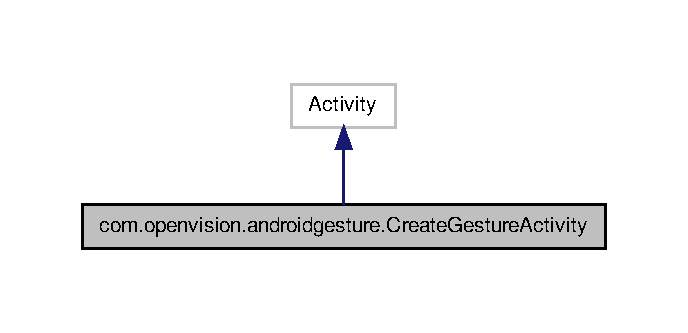
\includegraphics[width=330pt]{classcom_1_1openvision_1_1androidgesture_1_1CreateGestureActivity__inherit__graph}
\end{center}
\end{figure}


\-Collaboration diagram for com.\-openvision.\-androidgesture.\-Create\-Gesture\-Activity\-:\nopagebreak
\begin{figure}[H]
\begin{center}
\leavevmode
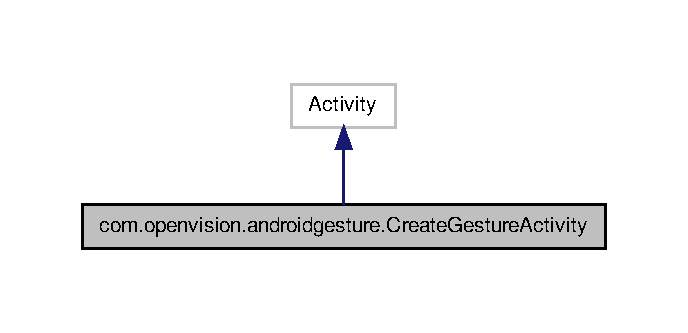
\includegraphics[width=330pt]{classcom_1_1openvision_1_1androidgesture_1_1CreateGestureActivity__coll__graph}
\end{center}
\end{figure}
\subsection*{\-Classes}
\begin{DoxyCompactItemize}
\item 
class {\bfseries \-Gestures\-Processor}
\end{DoxyCompactItemize}
\subsection*{\-Public \-Member \-Functions}
\begin{DoxyCompactItemize}
\item 
\hypertarget{classcom_1_1openvision_1_1androidgesture_1_1CreateGestureActivity_ace3259b9154231c56e426e7656cf72b1}{void {\bfseries add\-Gesture} (\-View v)}\label{classcom_1_1openvision_1_1androidgesture_1_1CreateGestureActivity_ace3259b9154231c56e426e7656cf72b1}

\item 
\hypertarget{classcom_1_1openvision_1_1androidgesture_1_1CreateGestureActivity_a13fa4290af05a5f24ef199ba3f3a09f5}{void {\bfseries cancel\-Gesture} (\-View v)}\label{classcom_1_1openvision_1_1androidgesture_1_1CreateGestureActivity_a13fa4290af05a5f24ef199ba3f3a09f5}

\item 
\hypertarget{classcom_1_1openvision_1_1androidgesture_1_1CreateGestureActivity_a90e2124a75b62cafab20d7ab63e9aea0}{native void {\bfseries add\-Gesture} (\-Array\-List$<$ \-Float $>$ location, \-Array\-List$<$ \-Long $>$ time, \-String name)}\label{classcom_1_1openvision_1_1androidgesture_1_1CreateGestureActivity_a90e2124a75b62cafab20d7ab63e9aea0}

\item 
\hypertarget{classcom_1_1openvision_1_1androidgesture_1_1CreateGestureActivity_a8c50fec91db3e2b2f4cc066a8fad1dcf}{native void {\bfseries set\-Directory} (\-String name)}\label{classcom_1_1openvision_1_1androidgesture_1_1CreateGestureActivity_a8c50fec91db3e2b2f4cc066a8fad1dcf}

\end{DoxyCompactItemize}
\subsection*{\-Protected \-Member \-Functions}
\begin{DoxyCompactItemize}
\item 
\hypertarget{classcom_1_1openvision_1_1androidgesture_1_1CreateGestureActivity_a4e81a9e8913ce9db0ca81aa8aab43a62}{void {\bfseries on\-Create} (\-Bundle saved\-Instance\-State)}\label{classcom_1_1openvision_1_1androidgesture_1_1CreateGestureActivity_a4e81a9e8913ce9db0ca81aa8aab43a62}

\item 
\hypertarget{classcom_1_1openvision_1_1androidgesture_1_1CreateGestureActivity_a0b5e3f5d97404c75edc228910d093af5}{void {\bfseries on\-Save\-Instance\-State} (\-Bundle out\-State)}\label{classcom_1_1openvision_1_1androidgesture_1_1CreateGestureActivity_a0b5e3f5d97404c75edc228910d093af5}

\item 
\hypertarget{classcom_1_1openvision_1_1androidgesture_1_1CreateGestureActivity_ac77cfb3c65018452e2e8951b6311492c}{void {\bfseries on\-Restore\-Instance\-State} (\-Bundle saved\-Instance\-State)}\label{classcom_1_1openvision_1_1androidgesture_1_1CreateGestureActivity_ac77cfb3c65018452e2e8951b6311492c}

\end{DoxyCompactItemize}
\subsection*{\-Package \-Functions}
\begin{DoxyCompactItemize}
\item 
\hypertarget{classcom_1_1openvision_1_1androidgesture_1_1CreateGestureActivity_a3ba84402193be3a929c761d54ca9f185}{void {\bfseries extract\-Gesture\-Info} ()}\label{classcom_1_1openvision_1_1androidgesture_1_1CreateGestureActivity_a3ba84402193be3a929c761d54ca9f185}

\end{DoxyCompactItemize}


\subsection{\-Detailed \-Description}
\begin{DoxyAuthor}{\-Author}
pi19404 
\end{DoxyAuthor}


\-The documentation for this class was generated from the following file\-:\begin{DoxyCompactItemize}
\item 
src/com/openvision/androidgesture/\-Create\-Gesture\-Activity.\-java\end{DoxyCompactItemize}

\hypertarget{classcom_1_1openvision_1_1androidgesture_1_1GestureLibraryInterface}{\section{com.\-openvision.\-androidgesture.\-Gesture\-Library\-Interface \-Class \-Reference}
\label{classcom_1_1openvision_1_1androidgesture_1_1GestureLibraryInterface}\index{com.\-openvision.\-androidgesture.\-Gesture\-Library\-Interface@{com.\-openvision.\-androidgesture.\-Gesture\-Library\-Interface}}
}


\-The documentation for this class was generated from the following file\-:\begin{DoxyCompactItemize}
\item 
src/com/openvision/androidgesture/\-Gesture\-Library\-Interface.\-java\end{DoxyCompactItemize}

\hypertarget{classGesturePoint}{\section{\-Gesture\-Point \-Class \-Reference}
\label{classGesturePoint}\index{\-Gesture\-Point@{\-Gesture\-Point}}
}
\subsection*{\-Public \-Member \-Functions}
\begin{DoxyCompactItemize}
\item 
\hypertarget{classGesturePoint_aff89af64ca5ad8ef7e0016d21a8d7355}{double {\bfseries get\-Time} ()}\label{classGesturePoint_aff89af64ca5ad8ef7e0016d21a8d7355}

\item 
\hypertarget{classGesturePoint_a85e2584a461cd0bb75e3e17612c3dbe6}{\-Point2f {\bfseries get\-Position} ()}\label{classGesturePoint_a85e2584a461cd0bb75e3e17612c3dbe6}

\end{DoxyCompactItemize}
\subsection*{\-Public \-Attributes}
\begin{DoxyCompactItemize}
\item 
\hypertarget{classGesturePoint_a1c868ede675da84e759c5b34f842a091}{\-Point2f {\bfseries position}}\label{classGesturePoint_a1c868ede675da84e759c5b34f842a091}

\item 
\hypertarget{classGesturePoint_acc9f7fa1c65945e4dc2a1b41cedd7e9b}{double {\bfseries time}}\label{classGesturePoint_acc9f7fa1c65945e4dc2a1b41cedd7e9b}

\end{DoxyCompactItemize}


\-The documentation for this class was generated from the following files\-:\begin{DoxyCompactItemize}
\item 
jni/\-Img\-App/\-Gesture\-Point.\-hpp\item 
jni/\-Img\-App/\-Gesture\-Point.\-cpp\end{DoxyCompactItemize}

\hypertarget{classcom_1_1openvision_1_1androidgesture_1_1OpenVisionGestureA}{\section{com.\-openvision.\-androidgesture.\-Open\-Vision\-Gesture\-A \-Class \-Reference}
\label{classcom_1_1openvision_1_1androidgesture_1_1OpenVisionGestureA}\index{com.\-openvision.\-androidgesture.\-Open\-Vision\-Gesture\-A@{com.\-openvision.\-androidgesture.\-Open\-Vision\-Gesture\-A}}
}


\-Inheritance diagram for com.\-openvision.\-androidgesture.\-Open\-Vision\-Gesture\-A\-:\nopagebreak
\begin{figure}[H]
\begin{center}
\leavevmode
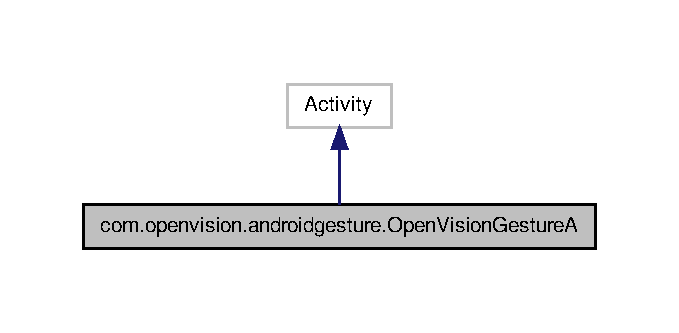
\includegraphics[width=326pt]{classcom_1_1openvision_1_1androidgesture_1_1OpenVisionGestureA__inherit__graph}
\end{center}
\end{figure}


\-Collaboration diagram for com.\-openvision.\-androidgesture.\-Open\-Vision\-Gesture\-A\-:\nopagebreak
\begin{figure}[H]
\begin{center}
\leavevmode
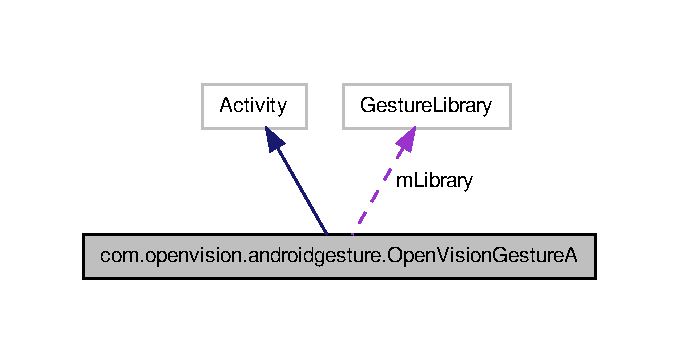
\includegraphics[width=326pt]{classcom_1_1openvision_1_1androidgesture_1_1OpenVisionGestureA__coll__graph}
\end{center}
\end{figure}
\subsection*{\-Public \-Member \-Functions}
\begin{DoxyCompactItemize}
\item 
\hypertarget{classcom_1_1openvision_1_1androidgesture_1_1OpenVisionGestureA_aaefb608bb2eaa60a776790d2bfadc5b2}{void {\bfseries add\-Gesture} (\-View v)}\label{classcom_1_1openvision_1_1androidgesture_1_1OpenVisionGestureA_aaefb608bb2eaa60a776790d2bfadc5b2}

\end{DoxyCompactItemize}
\subsection*{\-Protected \-Member \-Functions}
\begin{DoxyCompactItemize}
\item 
\hypertarget{classcom_1_1openvision_1_1androidgesture_1_1OpenVisionGestureA_a6aac46c9881523b42753a5dd8b9c9af6}{void {\bfseries on\-Create} (\-Bundle saved\-Instance\-State)}\label{classcom_1_1openvision_1_1androidgesture_1_1OpenVisionGestureA_a6aac46c9881523b42753a5dd8b9c9af6}

\item 
\hypertarget{classcom_1_1openvision_1_1androidgesture_1_1OpenVisionGestureA_ad03964962b8011fedae6cdfcf2fffb28}{void {\bfseries on\-Activity\-Result} (int request\-Code, int result\-Code, \-Intent data)}\label{classcom_1_1openvision_1_1androidgesture_1_1OpenVisionGestureA_ad03964962b8011fedae6cdfcf2fffb28}

\end{DoxyCompactItemize}
\subsection*{\-Package \-Attributes}
\begin{DoxyCompactItemize}
\item 
\hypertarget{classcom_1_1openvision_1_1androidgesture_1_1OpenVisionGestureA_a2b0b06802f0a20591f9bff2ac648fb5b}{\-Gesture\-Library {\bfseries m\-Library}}\label{classcom_1_1openvision_1_1androidgesture_1_1OpenVisionGestureA_a2b0b06802f0a20591f9bff2ac648fb5b}

\end{DoxyCompactItemize}


\-The documentation for this class was generated from the following file\-:\begin{DoxyCompactItemize}
\item 
src/com/openvision/androidgesture/\-Open\-Vision\-Gesture\-A.\-java\end{DoxyCompactItemize}

\hypertarget{classcom_1_1openvision_1_1androidgesture_1_1R}{\section{com.\-openvision.\-androidgesture.\-R \-Class \-Reference}
\label{classcom_1_1openvision_1_1androidgesture_1_1R}\index{com.\-openvision.\-androidgesture.\-R@{com.\-openvision.\-androidgesture.\-R}}
}
\subsection*{\-Classes}
\begin{DoxyCompactItemize}
\item 
class {\bfseries attr}
\item 
class {\bfseries color}
\item 
class {\bfseries dimen}
\item 
class {\bfseries drawable}
\item 
class {\bfseries id}
\item 
class {\bfseries layout}
\item 
class {\bfseries string}
\end{DoxyCompactItemize}


\-The documentation for this class was generated from the following file\-:\begin{DoxyCompactItemize}
\item 
gen/com/openvision/androidgesture/\-R.\-java\end{DoxyCompactItemize}

\hypertarget{classUniStrokeGesture}{\section{\-Uni\-Stroke\-Gesture \-Class \-Reference}
\label{classUniStrokeGesture}\index{\-Uni\-Stroke\-Gesture@{\-Uni\-Stroke\-Gesture}}
}
\subsection*{\-Public \-Attributes}
\begin{DoxyCompactItemize}
\item 
\hypertarget{classUniStrokeGesture_a8cc074d20ec291f5339c6633457ac6d9}{vector$<$ vector$<$ \hyperlink{classGesturePoint}{\-Gesture\-Point} $>$ $>$ {\bfseries \-\_\-gesture\-Point}}\label{classUniStrokeGesture_a8cc074d20ec291f5339c6633457ac6d9}

\item 
\hypertarget{classUniStrokeGesture_adc3efd8fae4f164168e5e767d576c661}{string {\bfseries \-\_\-name}}\label{classUniStrokeGesture_adc3efd8fae4f164168e5e767d576c661}

\end{DoxyCompactItemize}


\-The documentation for this class was generated from the following file\-:\begin{DoxyCompactItemize}
\item 
jni/\-Img\-App/\-Uni\-Stroke\-Gesture.\-hpp\end{DoxyCompactItemize}

\hypertarget{classUniStrokeGestureRecognizer}{\section{\-Uni\-Stroke\-Gesture\-Recognizer \-Class \-Reference}
\label{classUniStrokeGestureRecognizer}\index{\-Uni\-Stroke\-Gesture\-Recognizer@{\-Uni\-Stroke\-Gesture\-Recognizer}}
}
\subsection*{\-Public \-Member \-Functions}
\begin{DoxyCompactItemize}
\item 
void \hyperlink{classUniStrokeGestureRecognizer_a17a223c7cfb8908655f099806b6ec0df}{save} (string name, vector$<$ \hyperlink{classGesturePoint}{\-Gesture\-Point} $>$ points)
\item 
void \hyperlink{classUniStrokeGestureRecognizer_ac3365379a09d89079ba0ac515f6376e3}{load} ()
\item 
void \hyperlink{classUniStrokeGestureRecognizer_a826b32deaa2eae9a81cda3ed29de05de}{set\-Path} (string name)
\end{DoxyCompactItemize}


\subsection{\-Member \-Function \-Documentation}
\hypertarget{classUniStrokeGestureRecognizer_ac3365379a09d89079ba0ac515f6376e3}{\index{\-Uni\-Stroke\-Gesture\-Recognizer@{\-Uni\-Stroke\-Gesture\-Recognizer}!load@{load}}
\index{load@{load}!UniStrokeGestureRecognizer@{\-Uni\-Stroke\-Gesture\-Recognizer}}
\subsubsection[{load}]{\setlength{\rightskip}{0pt plus 5cm}void {\bf \-Uni\-Stroke\-Gesture\-Recognizer\-::load} (
\begin{DoxyParamCaption}
{}
\end{DoxyParamCaption}
)}}\label{classUniStrokeGestureRecognizer_ac3365379a09d89079ba0ac515f6376e3}
\-The functions loads all the gesture templates \hypertarget{classUniStrokeGestureRecognizer_a17a223c7cfb8908655f099806b6ec0df}{\index{\-Uni\-Stroke\-Gesture\-Recognizer@{\-Uni\-Stroke\-Gesture\-Recognizer}!save@{save}}
\index{save@{save}!UniStrokeGestureRecognizer@{\-Uni\-Stroke\-Gesture\-Recognizer}}
\subsubsection[{save}]{\setlength{\rightskip}{0pt plus 5cm}void {\bf \-Uni\-Stroke\-Gesture\-Recognizer\-::save} (
\begin{DoxyParamCaption}
\item[{string}]{dir, }
\item[{vector$<$ {\bf \-Gesture\-Point} $>$}]{points}
\end{DoxyParamCaption}
)}}\label{classUniStrokeGestureRecognizer_a17a223c7cfb8908655f099806b6ec0df}
function that stores the \-Gesture to a specified directory \hypertarget{classUniStrokeGestureRecognizer_a826b32deaa2eae9a81cda3ed29de05de}{\index{\-Uni\-Stroke\-Gesture\-Recognizer@{\-Uni\-Stroke\-Gesture\-Recognizer}!set\-Path@{set\-Path}}
\index{set\-Path@{set\-Path}!UniStrokeGestureRecognizer@{\-Uni\-Stroke\-Gesture\-Recognizer}}
\subsubsection[{set\-Path}]{\setlength{\rightskip}{0pt plus 5cm}void {\bf \-Uni\-Stroke\-Gesture\-Recognizer\-::set\-Path} (
\begin{DoxyParamCaption}
\item[{string}]{name}
\end{DoxyParamCaption}
)}}\label{classUniStrokeGestureRecognizer_a826b32deaa2eae9a81cda3ed29de05de}
set the name of the template gesture directory 

\-The documentation for this class was generated from the following files\-:\begin{DoxyCompactItemize}
\item 
jni/\-Img\-App/\-Uni\-Stroke\-Gesture\-Recognizer.\-hpp\item 
jni/\-Img\-App/\-Uni\-Stroke\-Gesture\-Recognizer.\-cpp\end{DoxyCompactItemize}

\printindex
\end{document}
